%
% 21-definition.tex -- Verschiedene Definitionsgebiete
%
% (c) 2026 Prof Dr Andreas Müller
%
\subsection{Fortsetzung einer Potenzreihe
\label{buch:analytisch:analytisch:subsection:potenzreihe}}
Wir betrachten eine holomorphe Funktion $f_1(z)$ mit der
Potenzreihenentwicklung
\[
f_1(z)
=
\sum_{k=0}^\infty a^1_k(z-z_1)^k
\]
um den Punkte $z_1$ mit Konvergenzradien $\varrho_1$.
Sei $z_2$ ein Punkt im Konvergenzkreis $D_1$ der Potenzreihe,
d.~h.  $ |z_2-z_1| < \varrho_1 $.
%
% fig-zweipunkte.tex -- analytische Fortsetzung für zwei Punkte
%
% (c) 2026 Prof Dr Andreas Müller
%
\begin{figure}
\centering
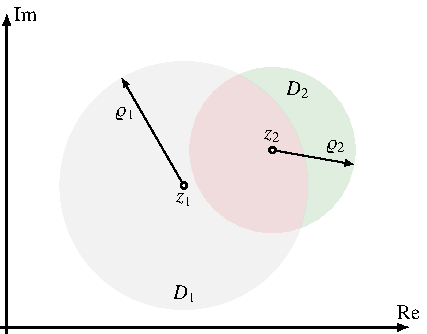
\includegraphics{chapters/040-analytisch/images/zweipunkte.pdf}
\caption{Die Potenzreihe einer auf dem Kreis um $z_1$ mit Radius
$\varrho_1$ definierte holomorphe Funktion $f_1(z)$ kann im Punkte
$z_2$ in eine neue Potenzreihe $f_2(z)$ mit Konvergenzradius
$\varrho_2$ entwickelt werden.
Im roten Teilgebiet stimmen die Funktionen überein.
Im grünen Teilgebiet ist die Funktion $f_2(z)$ die einzig mögliche
holomorphe Erweiterung der Funktion $f_1(z)$.
\label{buch:analytisch:fig:zweipunkte}}
\end{figure}

%

Durch rein algebraische Manipulationen können wir die Funktionen
$f_1(z)$ in eine Potenzreihe um den Punkte $z_2$ entwickeln.
Dazu schreiben wir $z=(z-z_2) + (z_2-z_1)$ und drücken
\begin{align}
f_1(z)
&=
\sum_{n=0}^\infty a^1_n(z-z_1)^n
\notag
\intertext{durch $z-z_2$ aus und erhalten}
&=
\sum_{n=0}^\infty a^1_n((z-z_2)+(z_2-z_1))^n.
\notag
\intertext{Mit dem Binomialsatz kann dies in}
&=
\sum_{n=0}^\infty \sum_{k+l=n} a^1_n\binom{n}{k}(z_2-z_1)^{l} (z-z_2)^k 
\notag
\intertext{expandiert werden.
Da die innere Summe endlich ist, lässt sich die Summationsreihenfolge
ändern:
}
&=
\sum_{k=0}^\infty
\Biggl(
\sum_{n=k}^\infty
a^1_n\binom{n}{n-k}
(z_2-z_1)^{n-k}
\Biggr)
(z-z_2)^k
\notag
\intertext{Die Binomialkoeffizienten können als Bruch geschrieben werden,
was}
&=
\sum_{k=0}^\infty
\Biggl(
\sum_{n=k}^\infty
a^1_n
\frac{n\cdot(n-1)\cdot\ldots\cdot(n-k+1)}{k!}
(z_2-z_1)^{n-k}
\Biggr)
(z-z_2)^k
\notag
\intertext{ergibt.
Der Nenner $k!$ in den Termen der inneren Summe hängt nicht vom
Summationsindex ab und kann daher vor die Summe genommen werden:}
&=
\sum_{k=0}^\infty
\frac{1}{k!}
\Biggl(
\sum_{n=k}^\infty
a^1_n
\bigl(
n\cdot(n-1)\cdot\ldots\cdot (n-k+1)
\bigr)
(z_2-z_1)^{n-k}
\Biggr)
(z-z_2)^k.
\notag
\intertext{Das Produkt $n\cdot(n-1)\cdot\ldots\cdot(n-k+1)z^{n-k}$
ist die $k$-te Ableitung von $z^n$.
Da $k$ für alle Terme der inneren Summe gleich ist, ist die
innere Summe die $k$-te Ableitung einer einfacheren Summe,
nämlich}
&=
\sum_{k=0}^\infty
\frac{1}{k!}
\frac{d^k}{dz_2^k}
\Biggl(
\sum_{n=k}^\infty
a^1_n
(z_2-z_1)^n
\Biggr)
(z-z_2)^k.
\notag
\intertext{Die innere Summe ist nichts anderes als die Funktion
$f_1(z_2)$:}
&=
\sum_{k=0}^\infty
\frac{1}{k!}
\frac{d^k}{dz_2^k}
f_1(z_2)
(z-z_2)^k.
\label{buch:analytisch:fortsetzung:eqn:taylor01}
\end{align}
Die letzte Reihe ist die Taylor-Reihe der Funktion $f_1$ an der
Stelle $z_2$.
Insbesondere gibt es eine holomorphe Funktion $f_2(z)$ mit 
Potenzreihenentwicklung im Punkt $z_2$ mit den Koeffizienten
\[
a^2_k
=
\frac{1}{k!}
\frac{d^kf_1(z_2)}{dz_2^k}.
\]
Die Potenzreihe konvergiert auf einem Kreis $D_2$ mit Radius $\varrho_2$
um den Punkte $z_2$ wie in Abbildung~\ref{buch:analytisch:fig:zweipunkte}
dargestellt.

Auf dem Schnittegebiet der beiden Konvergenzkreise, in der
Abbildung~\ref{buch:analytisch:fig:zweipunkte}
rot hervorgehoben, stimmen die Funktionen $f_1(z)$ und $f_2(z)$
überein.
Es ist aber gut möglich, dass der Konvergenzkreis von $f_2(z)$
Punkte enthält, die nicht im Konvergenzkreis von $f_1(z)$ liegen.
Die Funktion $f_2(z)$ definiert eine Fortsetzung der Funktion 
$f_1(z)$ in das in der 
Abbildung~\ref{buch:analytisch:fig:zweipunkte}
grün dargestellte Gebiet.
Diese Erweiterung auf die Vereinigung $D_1\cup D_2$ der beiden
Konvergenzkreise ist eindeutig bestimmt.

\begin{beispiel}
Die Funktion 
\[
f(z) = \frac{1}{1-z}
\]
hat um den Punkt $z_1=0$ die geometrische Reihe
\[
f_1(z)
=
\sum_{k=0}^\infty z^k
\]
mit Konvergenzradius $1$ als Potenzreihe.
Der Punkt $z_2=\frac12i$ liegt in diesem Konvergenzkreis.
Die Entwicklung um $z_2$ ist
\begin{align*}
f_2(z)
&=
\frac{1}{1-z+\frac12i-\frac12i}
=
\frac{1}{1+\frac12i-(z-\frac12i)}
=
\frac{1}{1-\frac{z-\frac12i}{1+\frac12i}}
\\
&=
\sum_{k=0}^\infty \biggl(\frac{z-\frac12i}{1+\frac12i}\biggr)^k
=
\sum_{k=0}^\infty \frac{1}{(1+\frac12i)^k}(z-\frac12i)^k,
\end{align*}
die für 
\[
\biggl|\frac{z-\frac12i}{1+\frac12i}\biggr|<1
\qquad\Rightarrow\qquad
\bigl|z-{\textstyle\frac12}i\bigr|
<
\bigl|1+{\textstyle\frac12}i\bigr|
=
\!\sqrt{1+\frac14}=\frac{\!\sqrt{5}}2 = \varrho_2
\]
konvergiert.
Der Konvergenzkreis der Potenzreihe $f_2(z)$ umfasst Punkte
ausserhalb des Konvergenzkreises von $f_1(z)$.
\end{beispiel}

Die Funktion des Beispiels ist überall in $\mathbb{C}$ ausser im Punkt
$z=1$ definiert und holomorph.
Das Beispiel illustriert, wie die Potenzreihe jeweils nur auf einem Kreis
um den Entwicklungspunkte konvergieren kann, der bis zur Singularität bei
$z=1$ reicht.

